\documentclass[11pt,a4paper]{article}
\usepackage[T1]{fontenc}
\usepackage[utf8]{inputenc}
\usepackage{lmodern}
\usepackage[margin=20mm]{geometry}
\usepackage{graphicx,float}
\usepackage[font=small,labelfont=bf]{caption}
\usepackage[hidelinks]{hyperref}
\graphicspath{{../figures/}}
\setlength{\parindent}{0pt}
\setlength{\parskip}{4pt}
\setlength{\intextsep}{8pt}

\begin{document}
\begin{center}
{\Large\bfseries DT081A --- Laboratory 3 Report\par}
Student: Jakob Obid\par
\texttt{obal2302@student.miun.se}\par
2026-11-06
\end{center}

\section{Introduction}
This lab studies how pixel values, colour channels, filters and spatial patterns affect digital images.

\section{Experimental Setup}
I used Python with NumPy, OpenCV and Matplotlib. Most experiments used the \texttt{ManWoman.png} image, which has a size of \(631 \times 475\) pixels. I worked with both colour and grayscale images and compared the results using graphs, images and measurements.

I also measured execution times to compare different methods and used PSNR to test noise reduction. For the morphology experiment, I created a separate binary image with different shapes. The settings for each experiment are given in the results sections.

\section{Results and Analysis}
\subsection{Human Perception of Color, Spatial Detail, and Gamma Correction}

\subsubsection*{Q1.1. Implement gamma correction and calculate the outputs for intensities 64, 128 and 192 using gamma = 2.0.}
\textbf{Answer:} I used gamma correction with gamma = 2.0. The outputs were 16, 64 and 144 for the three input values. The values were converted to integers for the final result.

\begin{table}[H]
\centering
\begin{tabular}{rr}
\hline
Input & Output \\
\hline
64 & 16 \\
128 & 64 \\
192 & 144 \\
\hline
\end{tabular}
\end{table}

\subsubsection*{Q1.2. Compare the image histograms before and after applying gamma = 2.2. Explain the relationship to nonlinear light perception.}
\textbf{Answer:} I applied gamma = 2.2 to the grayscale image. The mean intensity fell from 95.28 to 46.25, and the histogram moved toward darker values (Figure~\ref{fig:gamma-comparison}). This shows how a nonlinear intensity change affects brightness, which relates to how the eye responds nonlinearly to light.

\begin{figure}[H]
\centering
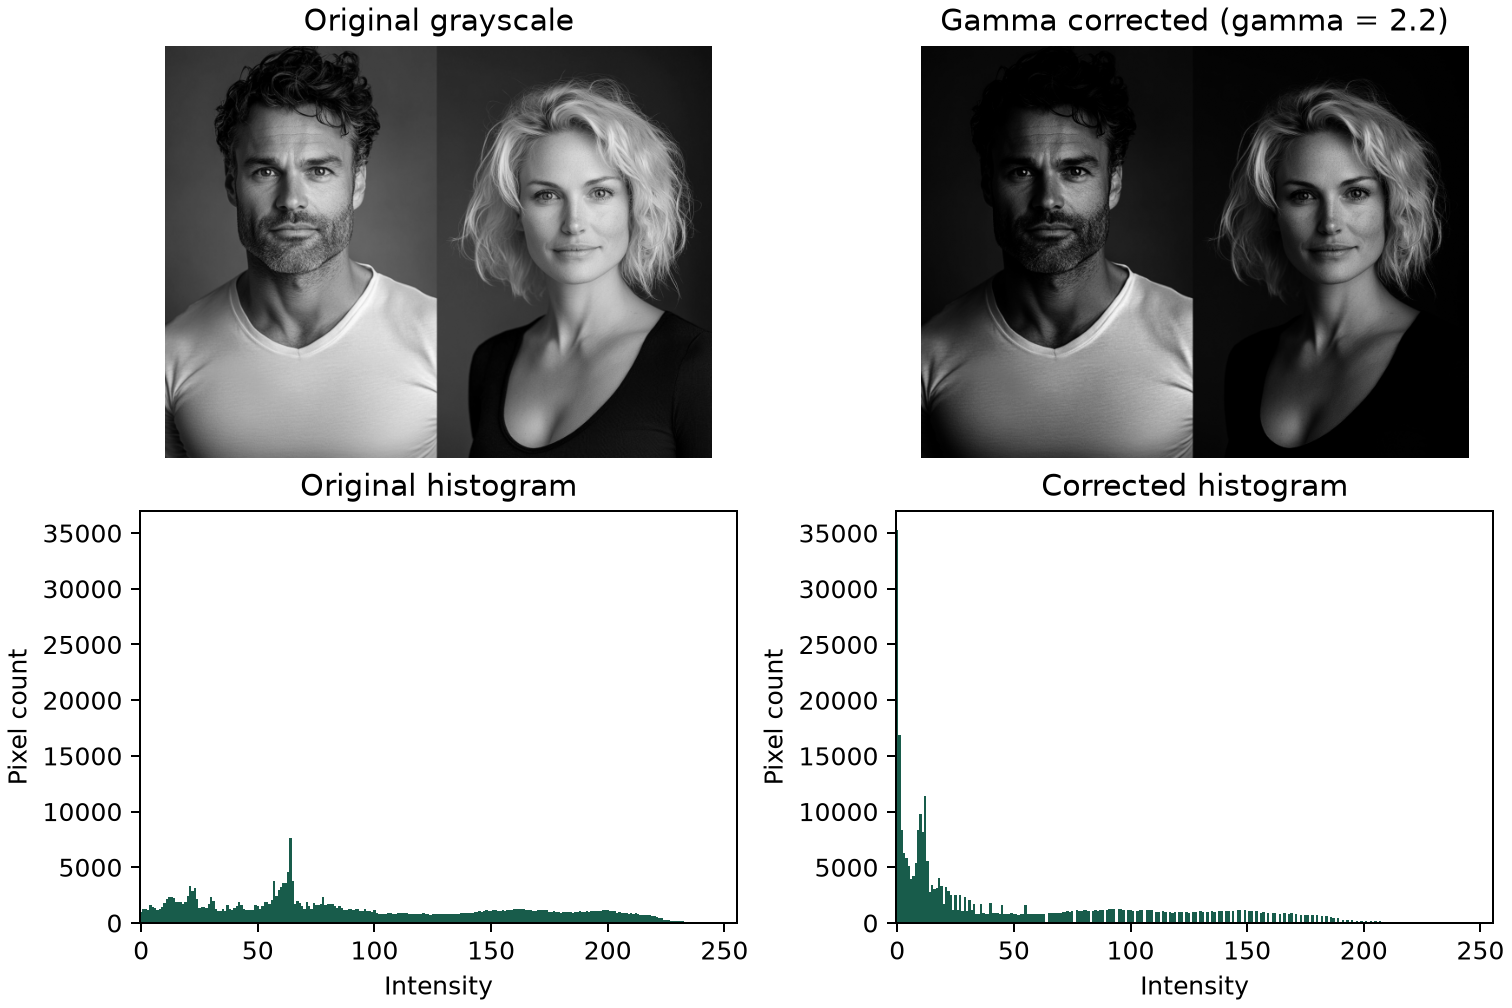
\includegraphics[width=0.92\linewidth]{section01_gamma_comparison.png}
\caption{Original grayscale image and gamma-corrected image (gamma = 2.2), with their intensity histograms.}
\label{fig:gamma-comparison}
\end{figure}

\subsection{Colorspaces (RGB and YCbCr)}

\subsubsection*{Q2.1. Compare the histogram spread of the Y channel versus R, G, and B channels. Why is the Y channel typically used for edge detection?}
\textbf{Answer:} The R channel had the widest histogram, with a standard deviation of 70.20. The Y channel had a standard deviation of 63.89, between R and the G/B channels. Y is useful for edge detection because it represents brightness in one channel, although it may miss boundaries that only differ in colour (Figure~\ref{fig:channel-histograms}).

\begin{figure}[H]
\centering
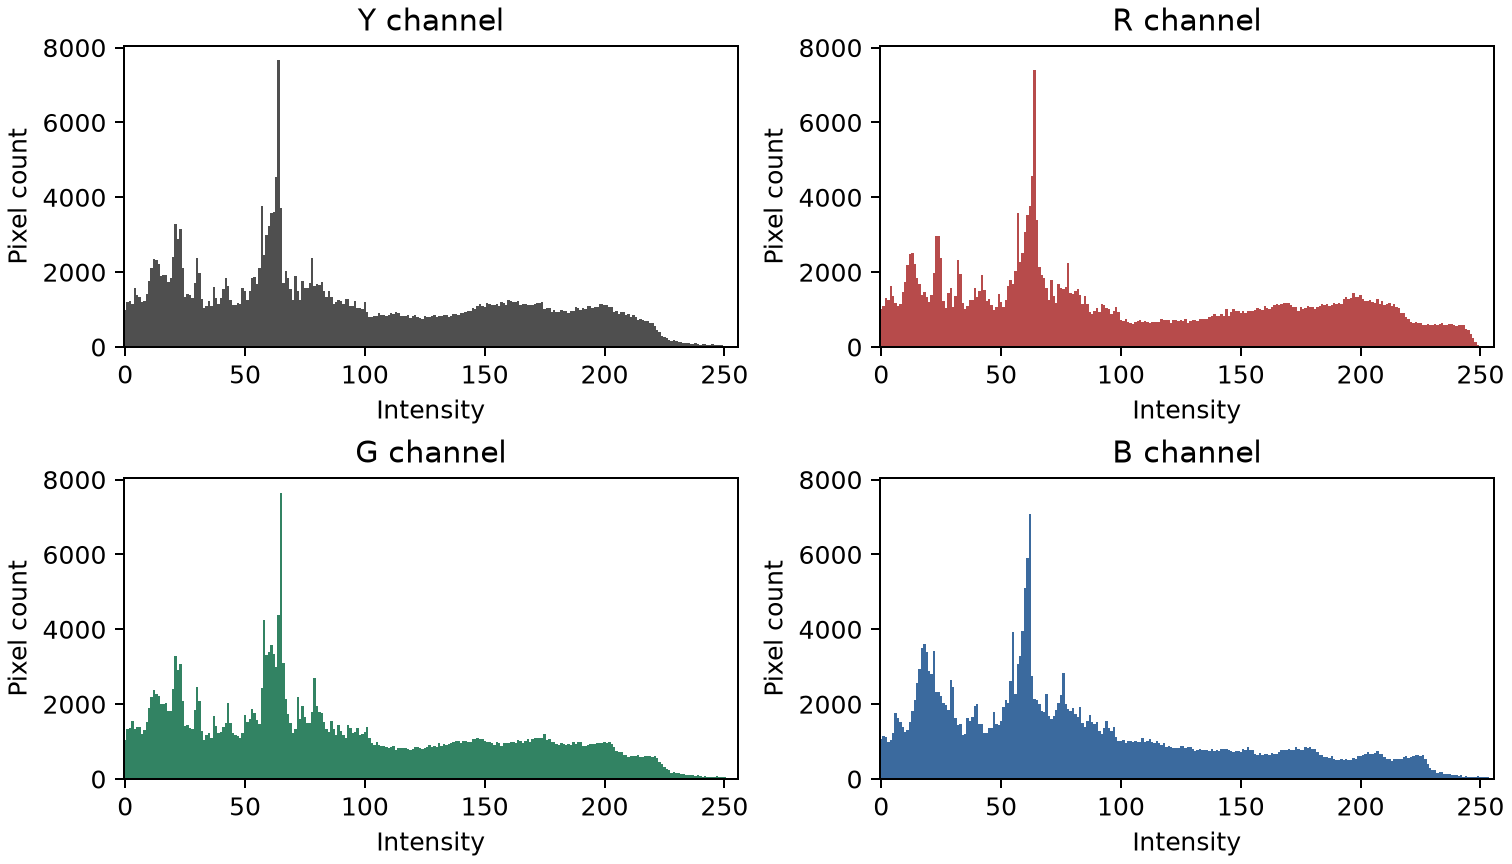
\includegraphics[width=0.90\linewidth]{section02_channel_histograms.png}
\caption{Intensity histograms of the Y, R, G and B channels.}
\label{fig:channel-histograms}
\end{figure}

\subsubsection*{Q2.2. If Cb and Cr channels are subsampled by a factor of 2, calculate the memory savings. At what point does this subsampling become visually noticeable if the subsampling factor is increased?}
\textbf{Answer:} Reducing both chroma dimensions by a factor of 2 saved about 50\% of the uncompressed channel storage. At factor 2, the image looked almost the same. At factors 4 and 8, colour edges became slightly softer when zoomed in (Figure~\ref{fig:chroma-subsampling}).

Each reduced chroma channel kept about one quarter of its samples. This reduced the total storage from three channel units to \(1 + 0.25 + 0.25 = 1.5\) units, saving about 50\%. For the actual image size, the saving was 50.06\%.

\begin{figure}[H]
\centering
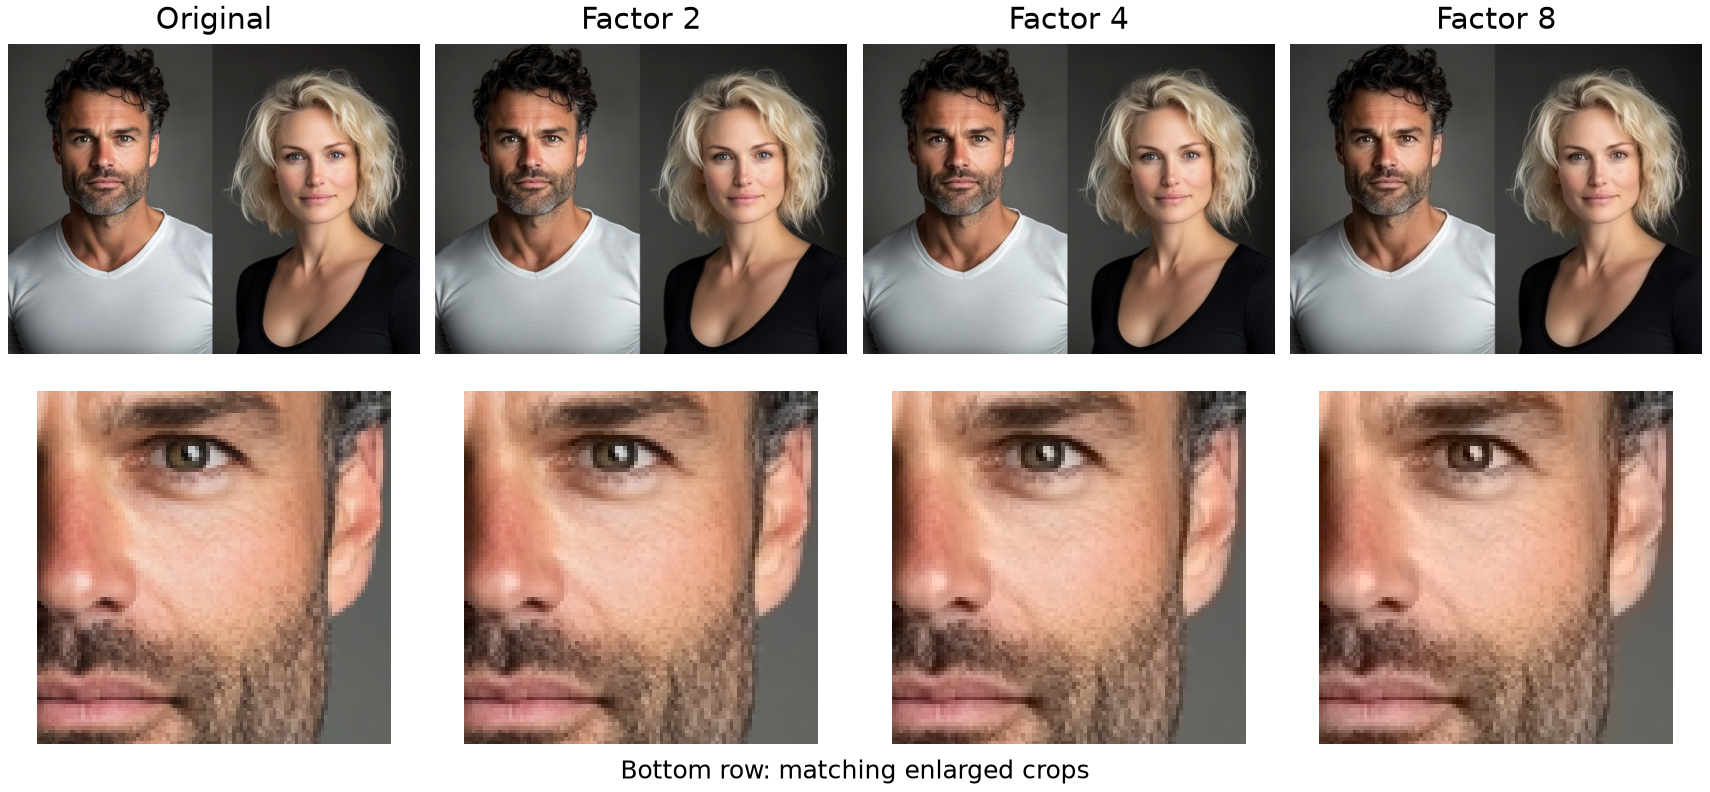
\includegraphics[width=0.95\linewidth]{section02_chroma_subsampling.png}
\caption{Chroma subsampling at factors 2, 4 and 8 compared with the original image.}
\label{fig:chroma-subsampling}
\end{figure}

\subsection{Image Quantization and Sampling}

\subsubsection*{Q3.1. Quantize the image to 4 bits and calculate the theoretical compression ratio achieved.}
\textbf{Answer:} I reduced each colour channel from 8 bits to 4 bits, giving 16 possible levels per channel. The theoretical compression ratio was 2:1, which means 50\% less storage if the values are packed. The colours became less smooth (Figure~\ref{fig:quantization}).

\subsubsection*{Q3.2. Plot the intensity distribution before and after 3-bit quantization. Explain the histogram's structure.}
\textbf{Answer:} I reduced the grayscale image to eight intensity levels. The new histogram had eight groups because every 32 input values were combined into one level. This removed some of the original intensity detail (Figure~\ref{fig:quantization}).

\begin{figure}[H]
\centering
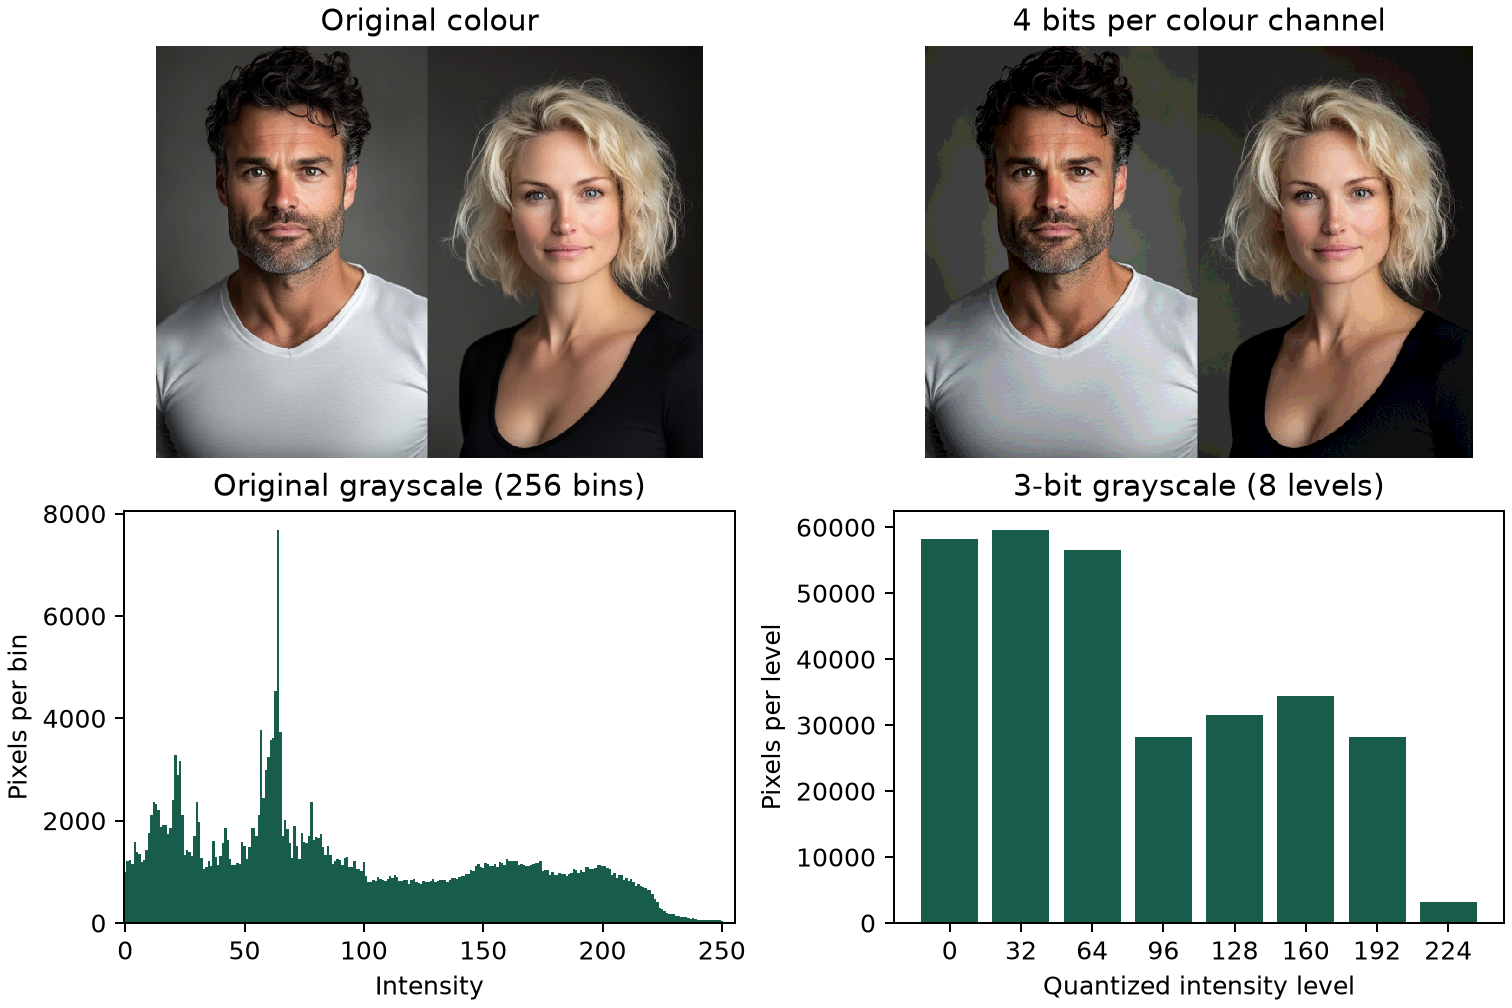
\includegraphics[width=0.92\linewidth]{section03_quantization.png}
\caption{Original and quantized images, with grayscale intensity histograms before and after 3-bit quantization.}
\label{fig:quantization}
\end{figure}

\subsection{Point Spread Functions and Convolution}

\subsubsection*{Q4.1. Compare the execution time of separable versus non-separable Gaussian filtering. When does separability provide significant advantage?}
\textbf{Answer:} I compared normal 2D Gaussian filtering with separable filtering using three kernel sizes. The measured times are shown in Table~\ref{tab:gaussian-times}. Both methods gave the same result within numerical precision. Separable filtering uses fewer kernel calculations for larger kernels, but the actual speed also depends on OpenCV.

\begin{table}[H]
\centering
\setcounter{table}{1}
\caption{Median Gaussian filtering times.}
\label{tab:gaussian-times}
\begin{tabular}{crr}
\hline
Kernel & Ordinary 2D (ms) & Separable (ms) \\
\hline
\(5\times5\) & 5.149 & 2.225 \\
\(11\times11\) & 5.148 & 2.922 \\
\(21\times21\) & 8.635 & 6.218 \\
\hline
\end{tabular}
\end{table}

Separable filtering was faster for all three tested kernel sizes.

\subsubsection*{Q4.2. Create a function that enhances an image's horizontal edges while suppressing vertical ones. Explain its structure.}
\textbf{Answer:} I used the Sobel filter with \texttt{dx=0} and \texttt{dy=1} to detect horizontal edges. It finds brightness changes from top to bottom, so horizontal boundaries appear stronger while vertical ones are weaker (Figure~\ref{fig:sobel-comparison}).

\subsubsection*{Q4.3. Show the result of applying the magnitude gradient kernel to the image.}
\textbf{Answer:} I combined the horizontal and vertical Sobel results to calculate the gradient magnitude. This highlighted edges in both directions (Figure~\ref{fig:sobel-comparison}).

\begin{figure}[H]
\centering
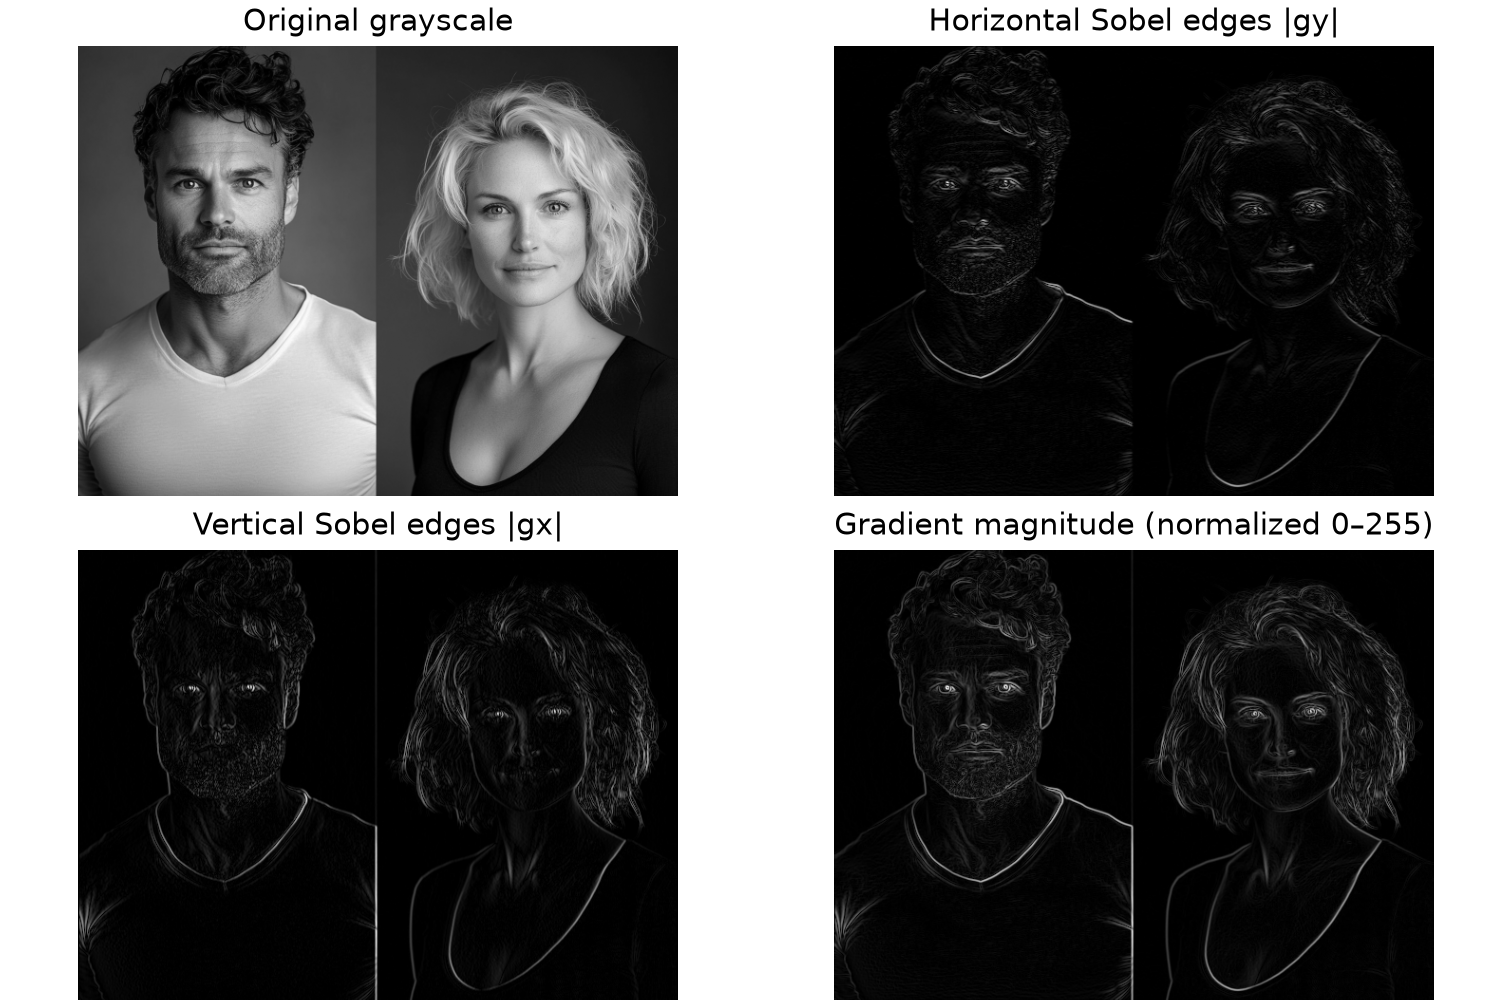
\includegraphics[width=0.92\linewidth]{section04_sobel_comparison.png}
\caption{Original grayscale image, horizontal and vertical Sobel edges, and the combined gradient magnitude.}
\label{fig:sobel-comparison}
\end{figure}

\subsection{Images as Stacked Vectors and Matrix Operations}

\subsubsection*{Q5.1. Implement image brightness and contrast adjustment using vector operations. Compare the computational efficiency with element-wise operations where nested loops are used, by measuring the execution time.}
\textbf{Answer:} I adjusted the image using a flattened vector and nested Python loops. Both methods produced the same result. The vector method took 2.72 ms, while the loops took 199.59 ms. The loop-to-vector time ratio was 73.45.

\begin{table}[H]
\centering
\begin{tabular}{lr}
\hline
Method & Time (ms) \\
\hline
Vectorized NumPy & 2.72 \\
Nested loops & 199.59 \\
\hline
\end{tabular}
\end{table}

\subsubsection*{Q5.2. Given a \(512\times512\) image, calculate the memory requirements for storing the explicit transformation matrix \(H\) for a \(3\times3\) convolution operation.}
\textbf{Answer:} A \(512\times512\) image has 262144 pixels, so the full matrix \(H\) would contain 68719476736 elements. It would need 256 GiB using float32 or 512 GiB using float64. This is too much memory for a simple \(3\times3\) convolution, so applying the small kernel directly is more practical.

\subsection{Pixel-Based Processing}

\subsubsection*{Q6.1. For your implementation, which is more efficient: direct computation or lookup tables? Quantify the difference.}
\textbf{Answer:} I applied the same logarithmic transformation using direct NumPy calculations and a lookup table. Both methods produced the same image. Direct computation took 9.83 ms, while the lookup table took 1.32 ms. The speed ratio was 7.45.

\begin{table}[H]
\centering
\begin{tabular}{lr}
\hline
Method & Average time (ms) \\
\hline
Direct NumPy & 9.83 \\
Lookup table & 1.32 \\
\hline
\end{tabular}
\end{table}

The time comparison excludes the one-time cost of building the lookup table.

\subsubsection*{Q6.2. Design a logarithmic transformation that enhances contrast in the middle intensity range while compressing shadows and highlights. Plot the transfer function.}
\textbf{Answer:} I used a logarithmic transformation with strength 3. The curve rises faster near middle gray and more slowly near black and white. For example, input values 112 and 144 became 98 and 157. This increases contrast between middle brightness values (Figure~\ref{fig:log-transform}).

\begin{figure}[H]
\centering
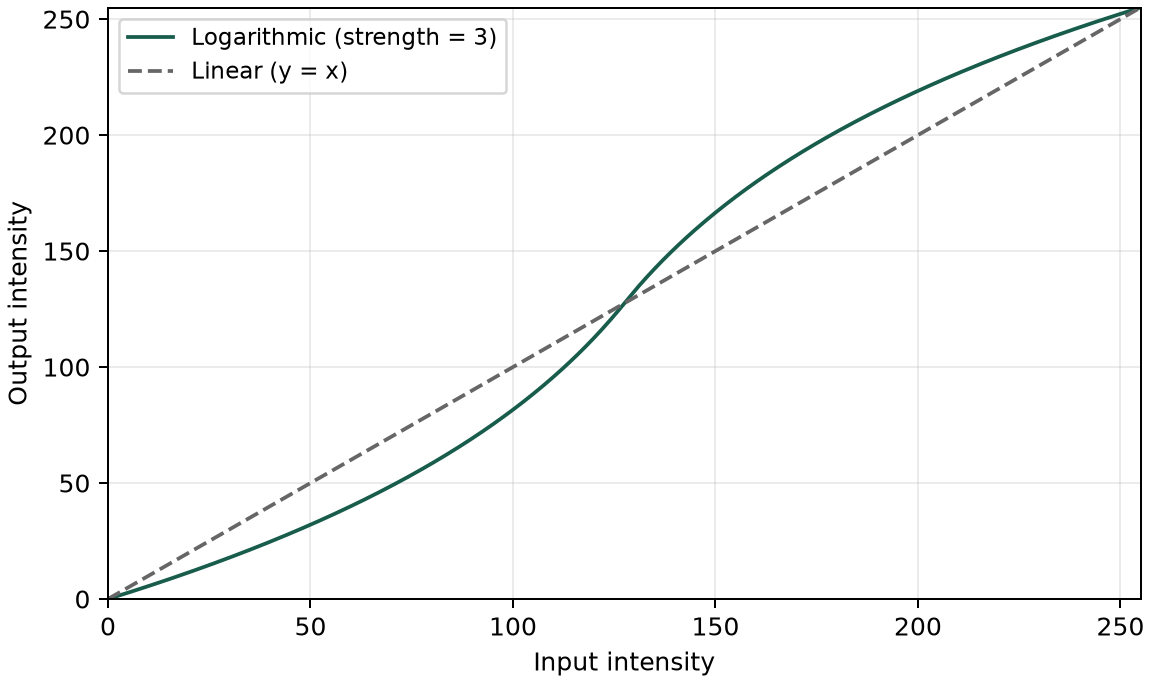
\includegraphics[width=0.78\linewidth]{section06_log_transform.png}
\caption{Logarithmic intensity transformation with increased middle-range contrast, compared with a linear transformation.}
\label{fig:log-transform}
\end{figure}

\subsection{Elementary Images and Linear Superposition}

\subsubsection*{Q7.1. Create four different elementary images of size \(16\times16\) using combinations of ramp, step, and sine basis vectors. How do they capture different image features?}
\textbf{Answer:} I created four \(16\times16\) images using ramp, step and sine vectors. Step \(\times\) Step made a sharp block, while Step \(\times\) Ramp and Ramp \(\times\) Step combined sharp boundaries with gradual changes. Sine \(\times\) Sine created a repeating pattern (Figure~\ref{fig:elementary-images}).

\subsubsection*{Q7.2. Select a simple geometric shape in an image of size \(16\times16\) and approximate it using only three elementary images by finding the best respective weights.}
\textbf{Answer:} I created a small triangle and approximated it using three elementary images. The weights were 0.5625 for Step \(\times\) Step, \(-0.4327\) for Step \(\times\) Ramp and 0.4327 for Ramp \(\times\) Step. The MSE was 0.0521. The approximation showed some of the triangular shape, but the diagonal edge was not exact (Figure~\ref{fig:elementary-images}).

\begin{figure}[H]
\centering
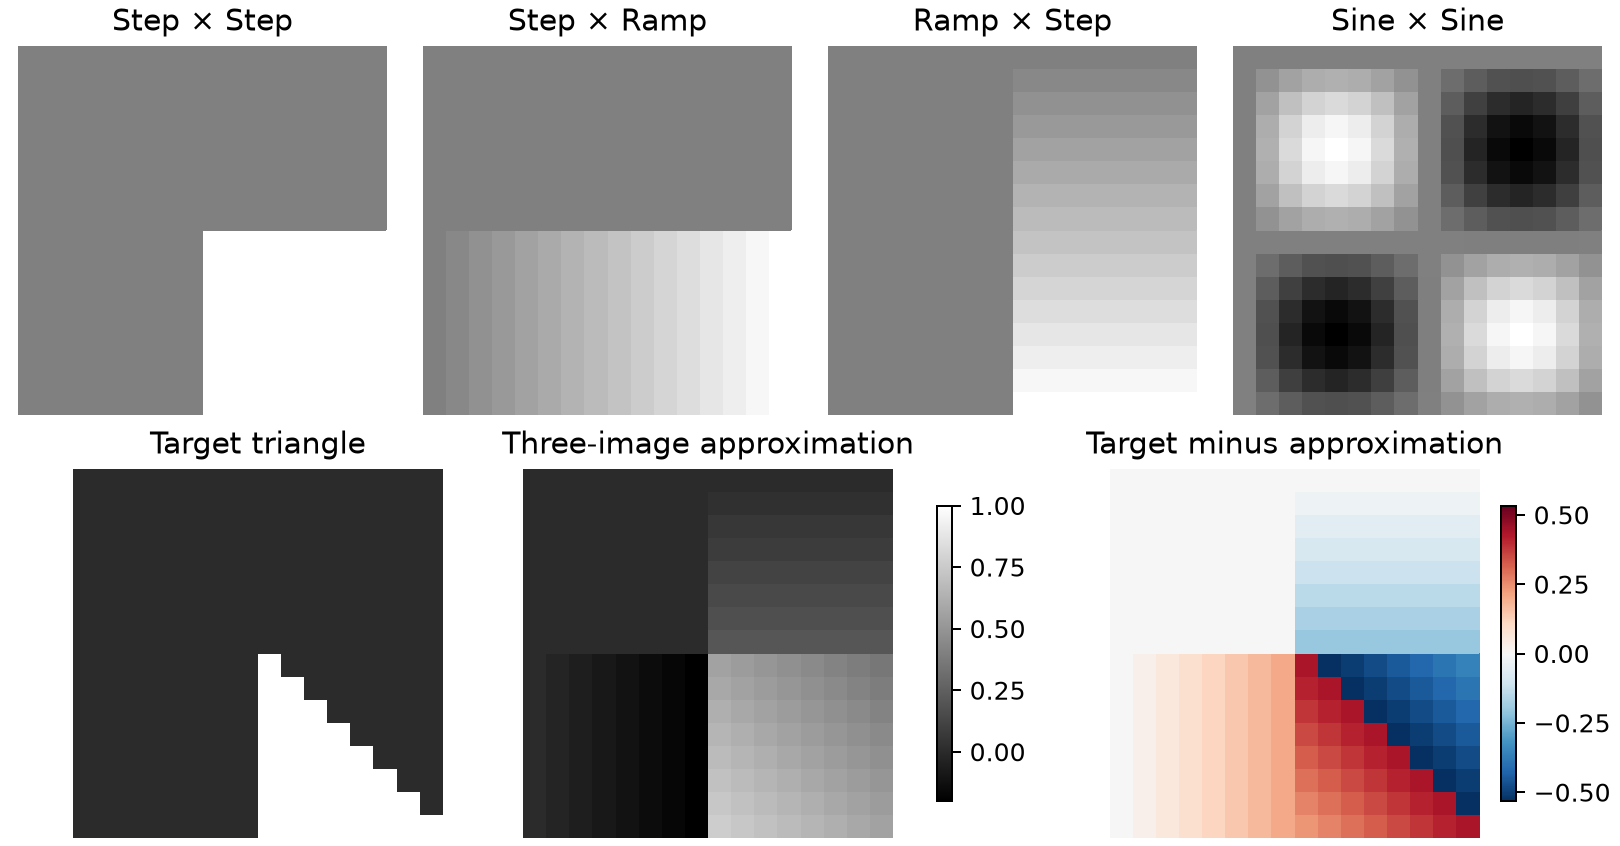
\includegraphics[width=0.95\linewidth]{section07_elementary_images.png}
\caption{Four elementary \(16\times16\) images and a triangle approximated using three weighted elementary images.}
\label{fig:elementary-images}
\end{figure}

\subsection{Transforms and Frequency Domain}

\subsubsection*{Q8.1. Apply the FFT to your image and identify the frequencies corresponding to dominant edges. Where are they located?}
\textbf{Answer:} I applied the 2D FFT to the grayscale image. The strongest values were near the centre, where the low frequencies are located. A horizontal streak in the spectrum is related to vertical edges, while a vertical streak is related to horizontal edges. The FFT shows these frequency patterns, but not the exact position of each edge (Figure~\ref{fig:fft-filters}).

\subsubsection*{Q8.2. Remove the high frequencies from the FFT, and inverse transform back to the spatial domain. Compare the result with the original image. What happens to the image content?}
\textbf{Answer:} I kept the frequencies inside a circle with a radius of 40 bins. After the inverse FFT, the main shapes were still visible, but smaller details and sharp edges became softer (Figure~\ref{fig:fft-filters}).

\subsubsection*{Q8.3. Remove the low frequencies from the FFT and inverse transform back to the spatial domain. Compare the result with the original image.}
\textbf{Answer:} I subtracted the low-pass image from the original to keep the high-frequency part. The result mainly showed edges and fine details, while smooth areas were close to zero (Figure~\ref{fig:fft-filters}).

\begin{figure}[H]
\centering
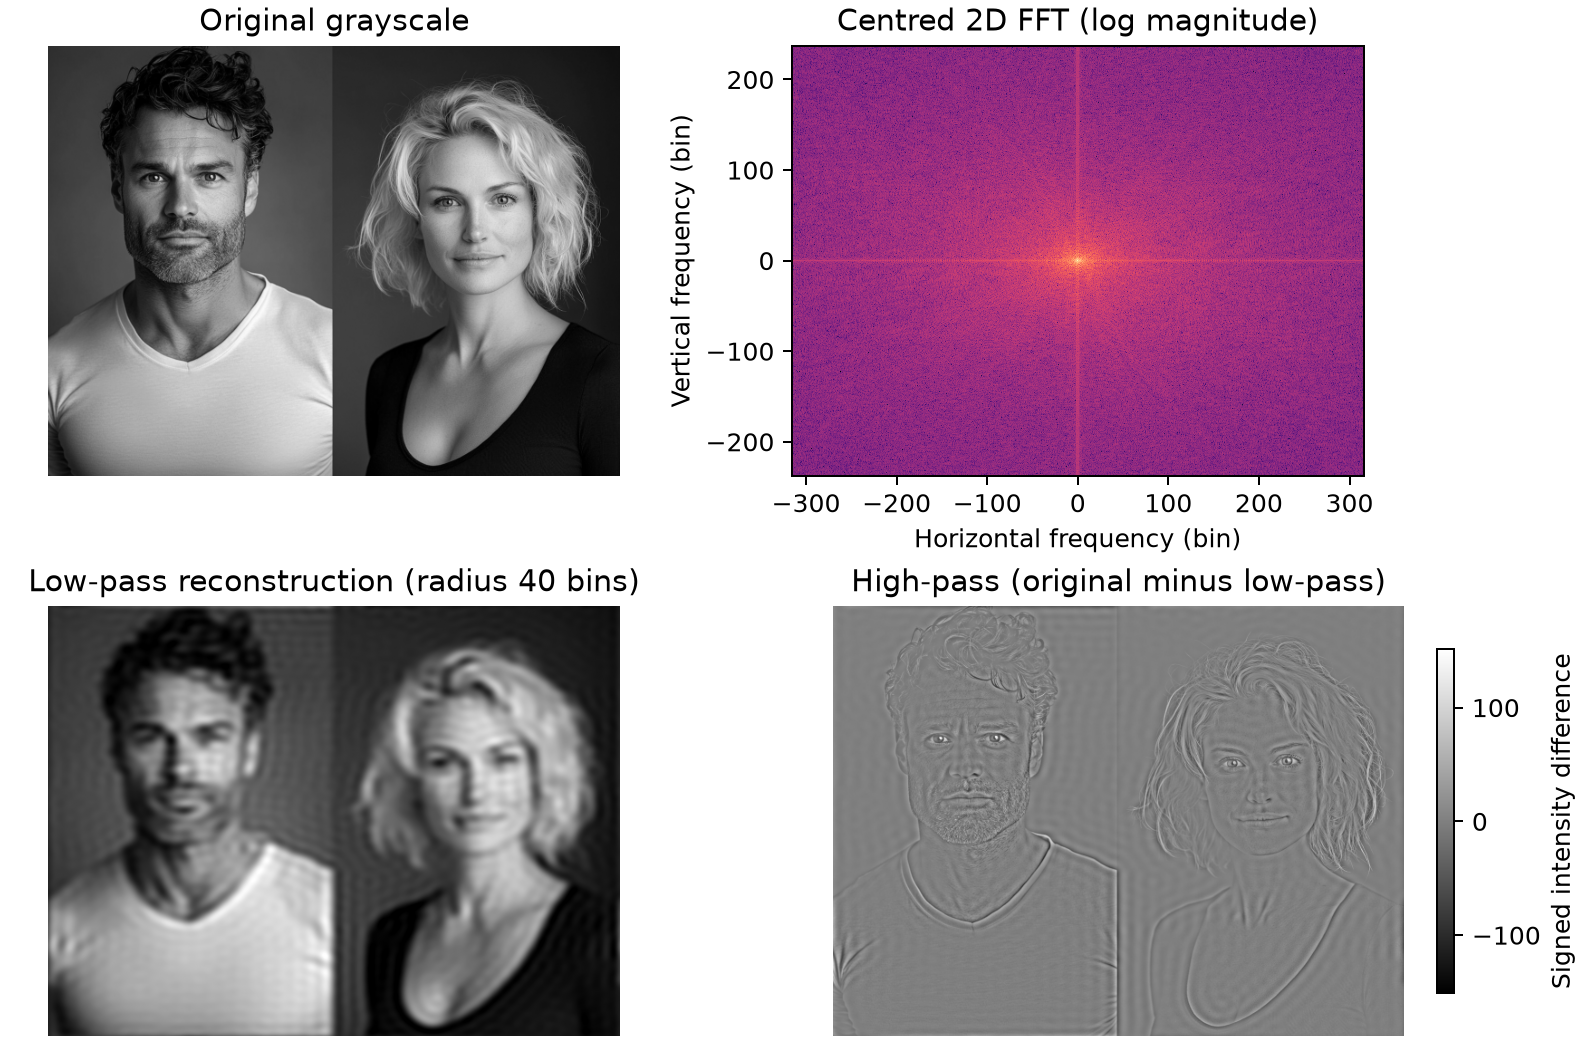
\includegraphics[width=0.95\linewidth]{section08_fft_filters.png}
\caption{Original image, 2D FFT magnitude spectrum, low-pass reconstruction and high-pass result.}
\label{fig:fft-filters}
\end{figure}

\subsection{Histograms and Image Enhancement}

\subsubsection*{Q9.1. Apply and plot the histogram and cumulative histogram functions to your image. What can be said about the image content based on the histogram and cumulative histogram?}
\textbf{Answer:} I calculated the histogram and cumulative histogram of the grayscale image. The most common intensity was 64, and 67.55\% of the pixels had an intensity of 127 or less. This shows that the image contains more dark and middle brightness values than very bright ones (Figure~\ref{fig:histogram-equalization}).

\subsubsection*{Q9.2. Apply histogram equalization to the image after reducing its contrast. Show the result and compare it with the original image. Validate using \texttt{cv2.equalizeHist()}.}
\textbf{Answer:} I reduced the contrast using a factor of 0.60. The intensity range became 51--202. After histogram equalization, the range increased to 0--254. The result had stronger contrast than the reduced image, but it did not restore the original pixel values. My CDF method differed from OpenCV by at most one intensity level (Figure~\ref{fig:histogram-equalization}).

\begin{figure}[H]
\centering
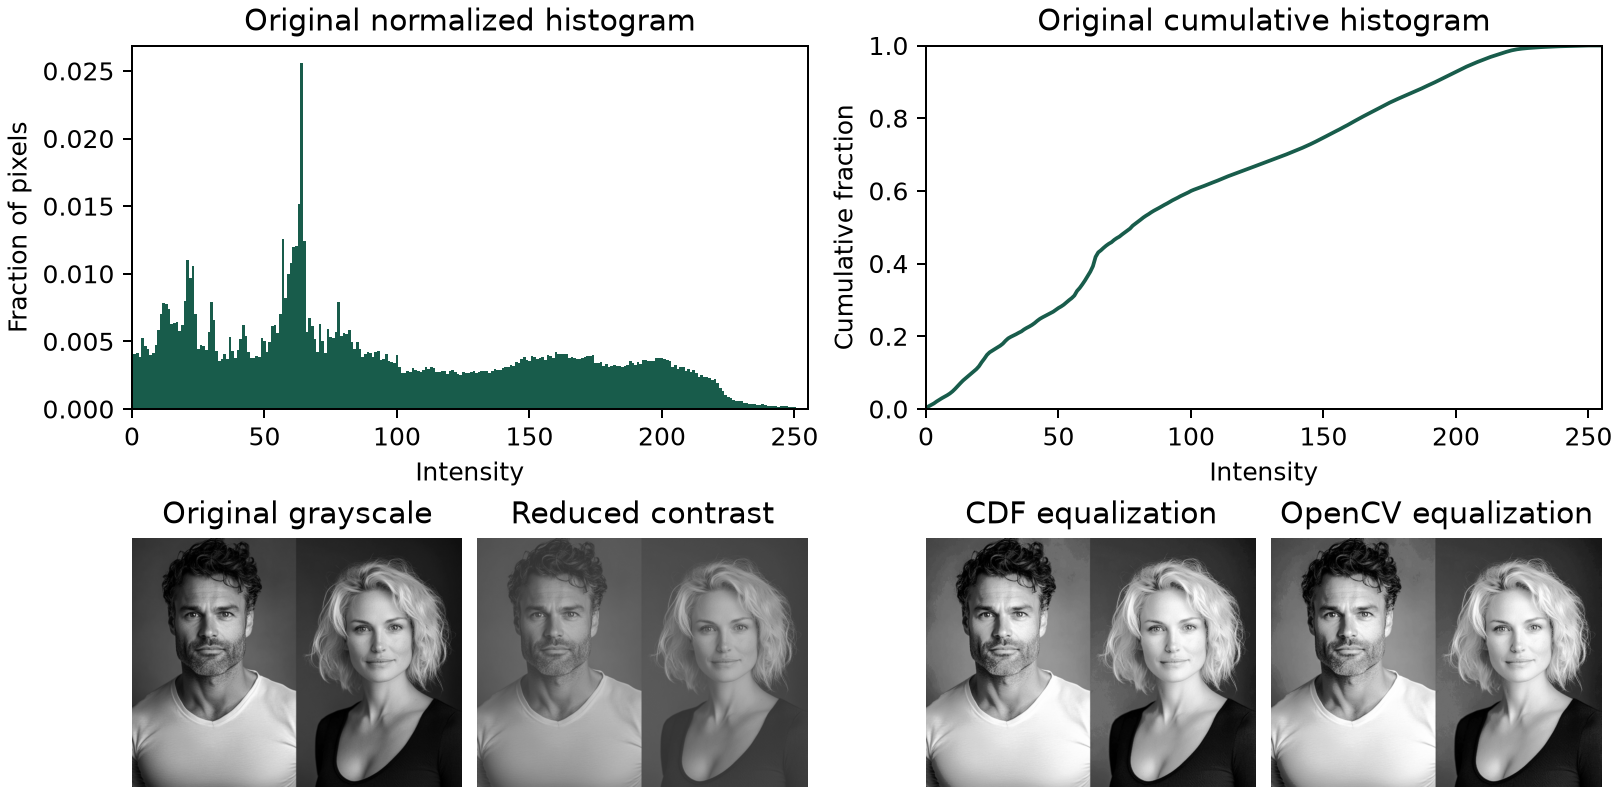
\includegraphics[width=0.95\linewidth]{section09_histogram_equalization.png}
\caption{Original histogram and CDF, with reduced-contrast and histogram-equalized images.}
\label{fig:histogram-equalization}
\end{figure}

\subsection{Noise and Noise Reduction}

\subsubsection*{Q10.1. Add noise to the filter and measure the PSNR of the results. Change the noise levels such that the same PSNR is achieved for both filters, and present the parameters used.}
\textbf{Answer:} I tested median and bilateral filtering with different Gaussian noise levels. With a noise standard deviation of 18.75 for the median filter and 27.00 for the bilateral filter, both results had a PSNR of about 29.00 dB. The bilateral filter handled stronger noise in this test.

\begin{table}[H]
\centering
\begin{tabular}{lrr}
\hline
Filter & Noise \(\sigma\) & Output PSNR (dB) \\
\hline
Median, \(3\times3\) & 18.75 & 29.00 \\
Bilateral, 9/75/75 & 27.00 & 29.01 \\
\hline
\end{tabular}
\end{table}

\subsubsection*{Q10.2. Compare the effectiveness of mean filtering versus median filtering for salt-and-pepper noise and Gaussian noise. Quantify the difference using PSNR.}
\textbf{Answer:} I compared mean and median filtering on both noise types. With Gaussian noise, mean filtering gave 28.40 dB compared with 27.10 dB for median filtering. With salt-and-pepper noise, median filtering worked better, reaching 35.02 dB compared with 27.09 dB for mean filtering (Figure~\ref{fig:noise-comparison}).

\begin{table}[H]
\centering
\begin{tabular}{lrr}
\hline
Noise & Mean (dB) & Median (dB) \\
\hline
Gaussian & 28.40 & 27.10 \\
Salt-and-pepper & 27.09 & 35.02 \\
\hline
\end{tabular}
\end{table}

\begin{figure}[H]
\centering
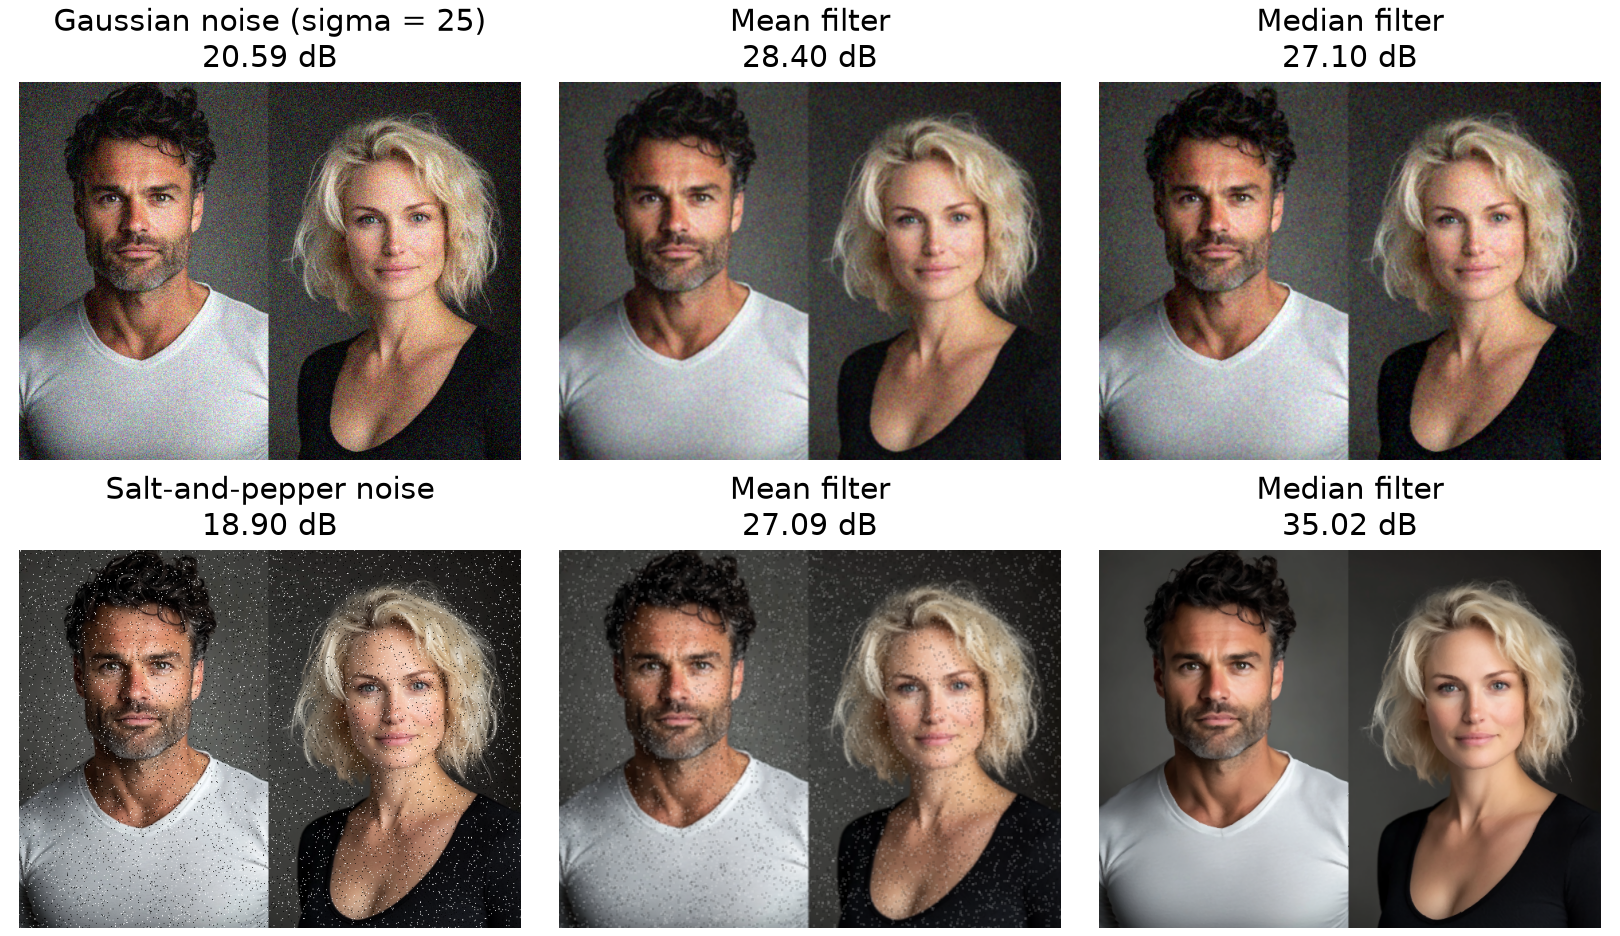
\includegraphics[width=0.95\linewidth]{section10_noise_comparison.png}
\caption{Mean and median filtering results for Gaussian and salt-and-pepper noise.}
\label{fig:noise-comparison}
\end{figure}

\subsection{Morphological Filtering}

\subsubsection*{Q11.1. Develop a sequence of morphological operations to detect and count objects in a binary image. Test with different object shapes.}
\textbf{Answer:} I created a binary image with a circle, a rectangle and a triangle. I also added four isolated white pixels. Opening and closing removed the small unwanted pixels, leaving three connected objects. I counted them using connected components (Figure~\ref{fig:morphology}).

See the code appendix for the object counting steps.

\subsubsection*{Q11.2. Compare the morphological gradient with the Sobel based gradient in Section 4 for edge detection. When is each method preferable?}
\textbf{Answer:} I compared the morphological gradient with the Sobel gradient. The morphological gradient used dilation minus erosion to highlight local boundaries. Sobel detected brightness changes using horizontal and vertical derivatives. Morphological filtering is useful for binary objects and shapes, while Sobel is useful for finding edges in grayscale images (Figure~\ref{fig:morphology}).

\begin{figure}[H]
\centering
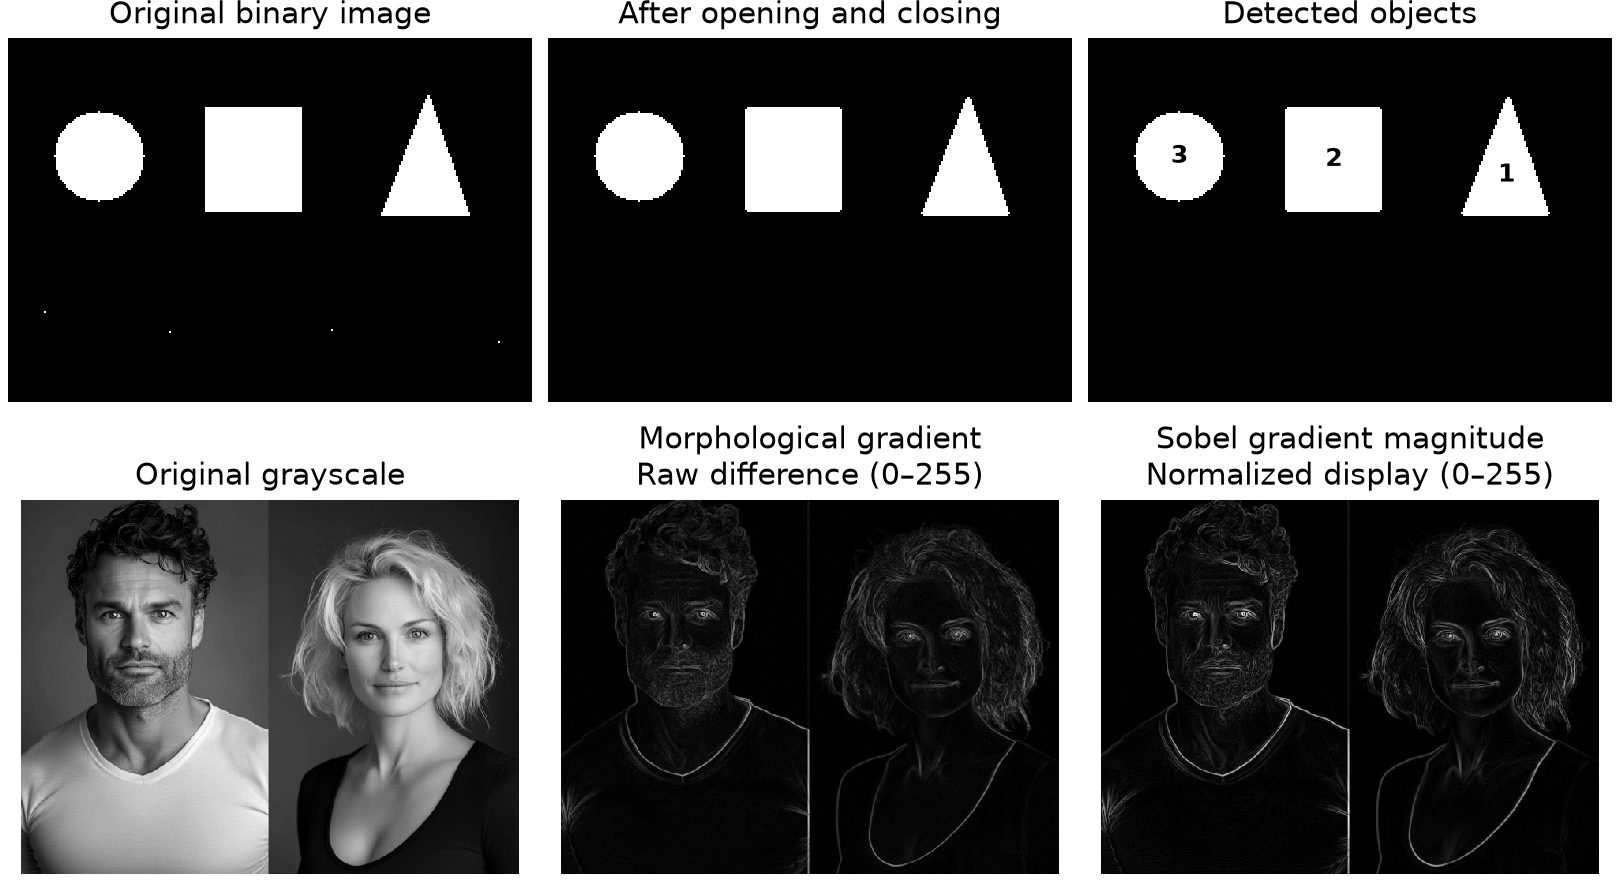
\includegraphics[width=0.95\linewidth]{section11_morphology.png}
\caption{Morphological object detection and comparison of morphological and Sobel gradients.}
\label{fig:morphology}
\end{figure}

\section{Discussion}
The results showed that reducing image information can save storage, but some details are lost. For example, stronger chroma subsampling made colour edges softer, while quantization reduced the number of intensity levels.

The timing tests showed that vector operations and lookup tables were much faster than the other methods tested. I also found that different noise types needed different filters. Mean filtering worked better for Gaussian noise, while median filtering worked better for salt-and-pepper noise.

The triangle approximation showed that three elementary images could not reproduce every detail. My histogram equalization was also very close to OpenCV's result, with a difference of at most one intensity level.

Overall, the experiments showed that different methods have different advantages depending on the task.

\section{Conclusion}
In this lab, I tested how image processing changes brightness, colour, detail and noise. The results showed that reducing image information can save space but also remove detail. Different filters worked better for different tasks, such as removing noise, detecting edges and counting objects. I learned that choosing the right method depends on what I want to preserve in the image.

\section*{Appendix: Code Snippets}
\textbf{Gamma correction}
\begin{verbatim}
def apply_gamma(image, gamma):
    normalized = image.astype(np.float32) / 255.0
    corrected_image = 255 * np.power(normalized, gamma)
    return np.uint8(corrected_image)
\end{verbatim}
The function scales the pixel values to 0--1, applies gamma and converts the result back to 8-bit values.

\textbf{FFT filtering}
\begin{verbatim}
cutoff = 40
mask = ideal_lowpass(gray.shape, cutoff)
F_low = F_shift * mask
low_pass = np.fft.ifft2(np.fft.ifftshift(F_low)).real
\end{verbatim}
The mask keeps the low frequencies, and the inverse FFT turns them back into an image.

\textbf{Morphological object counting}
\begin{verbatim}
opened = cv2.morphologyEx(binary, cv2.MORPH_OPEN, cross_kernel)
cleaned = cv2.morphologyEx(opened, cv2.MORPH_CLOSE, disk_kernel)
before, _ = cv2.connectedComponents(binary, connectivity=8)
n, labels, stats, centroids = cv2.connectedComponentsWithStats(
    cleaned, connectivity=8
)
object_count = n - 1  # Label zero is the background.
\end{verbatim}
Opening and closing clean the binary image before the connected objects are counted.
\end{document}
